\chapter{Protótipos estruturais}\label{cap:prototipos}

% ==============================================================================
% INTRODUÇÃO 
% ==============================================================================

A análise independente dos campos de precipitação total (Capítulo~\ref{cap:resultados_tp}) e vento a 10 metros (Capítulo~\ref{cap:resultados_wind10}) desenvolvida nos capítulos anteriores revelou que ambas as variáveis exibem transformações estruturais profundas e qualitativamente distintas ao longo do ciclo de vida ciclônico, com uma reorganização espacial que depende da intensidade dinâmica do sistema.

No entanto, a descrição separada de cada campo não permite quantificar a diferenciação espacial conjunta entre os campos de circulação e precipitação em um único quadro de referência. 
Para fechar essa lacuna analítica, o presente capítulo introduz uma representação sintética denominada \textit{protótipo estrutural acoplado}: uma visualização integrada que sobrepõe, no mesmo domínio lagrangiano, os campos de densidade de probabilidade espacial (PDF) e os padrões EOF dominantes de ambas as variáveis simultaneamente.

Cada protótipo combina quatro camadas de informação geométrica: (i) os contornos PDFe dos quartis 75 e 90 para a precipitação (azul) e o vento (vermelho), que mapeiam as zonas de maior concentração probabilística de máximos; (ii) as linhas de carga positiva (sólida) e negativa (tracejada) do primeiro modo EOF para ambas as variáveis (verde para precipitação, laranja para vento), que identificam os padrões espaciais de maior variabilidade; e (iii) as coordenadas modais ($\Delta x$, $\Delta y$) de cada campo em relação ao centro do vórtice (0,0), representadas por estrelas. O domínio de análise corresponde ao quadro lagrangiano de $20^{\circ} \times 20^{\circ}$ centrado no núcleo ciclônico, delimitado por uma máscara circular de raio $9{,}5^{\circ}$ que recorta o perímetro de cada painel. Apresentam-se duas versões: a População Global (Fig.~\ref{fig:prototipo_global}) e o subconjunto de ciclones de alta vorticidade p90 (Fig.~\ref{fig:prototipo_p90}), organizadas em uma matriz de $3 \times 4$ painéis (regiões $\times$ fases evolutivas), facilitando a leitura comparativa da diferenciação entre campos ao longo de todo o ciclo de vida.

% ==============================================================================
\section{População Global}\label{sec:prototipo_global}
% ==============================================================================

\begin{figure}[H]
\centering
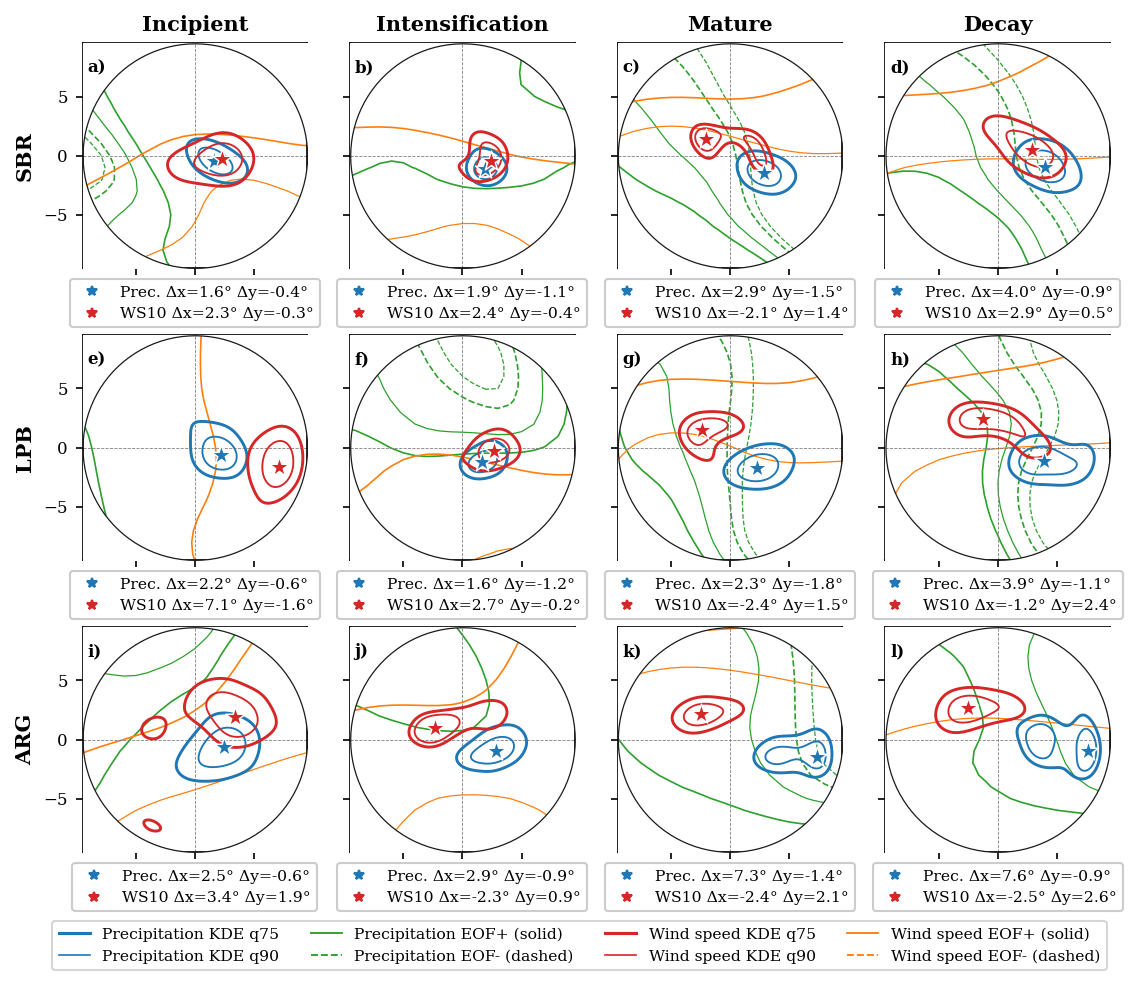
\includegraphics[width=\textwidth]{images/prototipos/prototipo_12panels_global.png}
\caption[Protótipos estruturais acoplados — População Global]{Protótipos estruturais acoplados para a População Global de ciclones extratropicais do Atlântico Sudoeste. Cada painel sobrepõe no domínio lagrangiano $20^{\circ} \times 20^{\circ}$ centrado no vórtice (0,0) os contornos PDFe dos quantis 75 e 90 de precipitação total (azul, linha grossa e fina respectivamente) e vento a 10 m (vermelho), juntamente com as cargas positivas (linha sólida) e negativas (linha tracejada) do EOF1 de precipitação (verde) e vento (laranja). As estrelas azul e vermelha indicam as coordenadas modais ($\Delta x$, $\Delta y$) de cada campo. A matriz organiza as regiões de ciclogênese em linhas (SBR, LPB, ARG) e as fases evolutivas em colunas (Incipiente, Intensificação, Maturidade, Declínio). A máscara circular delimita o domínio a um raio de $9{,}5^{\circ}$.}
\label{fig:prototipo_global}
\end{figure}

A Figura~\ref{fig:prototipo_global} apresenta os protótipos estruturais acoplados para a População Global. Cada painel integra em um único espaço de representação a geometria probabilística dos máximos de ambas as variáveis com os padrões de maior variabilidade explicada (EOF1), proporcionando uma leitura simultânea da localização preferencial dos forçantes dinâmicos de precipitação e circulação ao longo do ciclo de vida. 

Esta figura foi construída a partir dos campos PDFe calculados sobre a grade lagrangiana fixa (Seção~\ref{subsec:kde_tp_global} para precipitação e Seção~\ref{sec:kde_espacial_global} para vento), combinados com o primeiro autovetor espacial das análises EOF independentes (Seção~\ref{sec:eof_tp} e Seção~\ref{sec:eof_wind10}, respectivamente). 
Os contornos de densidade foram suavizados mediante um filtro gaussiano ($\sigma = 2$) antes de traçar os níveis correspondentes aos quantis 75 e 90 da distribuição acumulada, seguindo o critério de região de maior densidade (HDR). 
Sua inclusão tem como propósito sintetizar, em uma visualização integrada, a coexistência espacial ou a diferenciação entre os campos de circulação e precipitação nos ciclones ordinários, estabelecendo a linha de base em relação à qual se comparará o subconjunto de alta vorticidade na seção seguinte.

Durante as fases incipiente e de intensificação (painéis a--f), os protótipos da População Global exibem um padrão de co-localização relativa entre os máximos de precipitação e vento. Em SBR (painéis a--b), os contornos PDFe de ambas as variáveis se sobrepõem parcialmente no entorno do quadrante oriental, com as modas de precipitação (estrela azul) e vento (estrela vermelha) separadas por apenas $0{,}5^{\circ}$--$1^{\circ}$ em latitude, enquanto as cargas do EOF1 de vento (laranja sólida) se estendem para o setor noroeste. Em LPB (painéis e--f), os núcleos de densidade de precipitação se situam ligeiramente a leste do centro, enquanto os de vento se posicionam a sudoeste durante a fase incipiente, com uma separação modal que oscila entre $4{,}9^{\circ}$ e $5{,}5^{\circ}$ na direção zonal. Em ARG (painéis i--j), o padrão é bimodal desde as etapas iniciais: o PDFe de vento se concentra a sudoeste do vórtice enquanto o de precipitação o faz a nordeste, antecipando a divergência estrutural que se consolida na maturidade. Esta co-localização parcial durante as fases iniciais reflete que, no regime médio, os forçantes frontais da WCB organizam ambos os campos no mesmo setor ativo do ciclone, antes que a diferenciação interna da estrutura ciclônica imponha geometrias distintas.

Ao transitar para a maturidade (painéis c, g, k) e o declínio (painéis d, h, l), a arquitetura do protótipo se modifica de maneira sistemática embora moderada na População Global. Os contornos PDFe de vento se deslocam para o setor noroeste e oeste, coerentemente com o aumento dos gradientes de pressão no flanco posterior do ciclone, enquanto os de precipitação se expandem difusamente para leste e sudeste. Esta separação, quantificada pela distância entre estrelas modais, atinge valores de até $5^{\circ}$--$7^{\circ}$ na direção zonal para SBR e LPB durante a maturidade (painéis c, g), aumentando no declínio. No entanto, tanto os contornos PDFe quanto as cargas EOF1 mantêm na População Global uma extensão espacial considerável, sem que nenhum campo colapse para uma geometria estreita e bem definida. Este comportamento difuso reflete a heterogeneidade estrutural inerente ao catálogo completo, onde a integração de ciclones com diferentes taxas de oclusão, profundidades de vórtice e ambientes termodinâmicos dilui o sinal espacial de qualquer subconjunto estruturalmente coerente.

A comparação regional revela assimetrias na dinâmica de separação. Em ARG (painéis i--l), a divergência entre os PDFe de vento e precipitação é a mais pronunciada desde as fases iniciais, com a moda de vento deslocada sistematicamente para sudoeste ($\Delta x < 0$, $\Delta y > 0$) enquanto a de precipitação mantém valores positivos em ambas as componentes. Este comportamento contrasta com SBR e LPB, onde a separação meridional é menor e a distribuição de precipitação é mais extensa, refletindo o maior acesso à umidade oceânica e a maior variabilidade de trajetórias das células de precipitação. Estas diferenças regionais são coerentes com os padrões individuais descritos nos capítulos anteriores e confirmam que a síntese estrutural do protótipo não média essas diferenças, mas as preserva na leitura integrada.

% ==============================================================================
\section{Subconjunto de alta vorticidade (p90)}\label{sec:prototipo_p90}
% ==============================================================================

\begin{figure}[H]
\centering
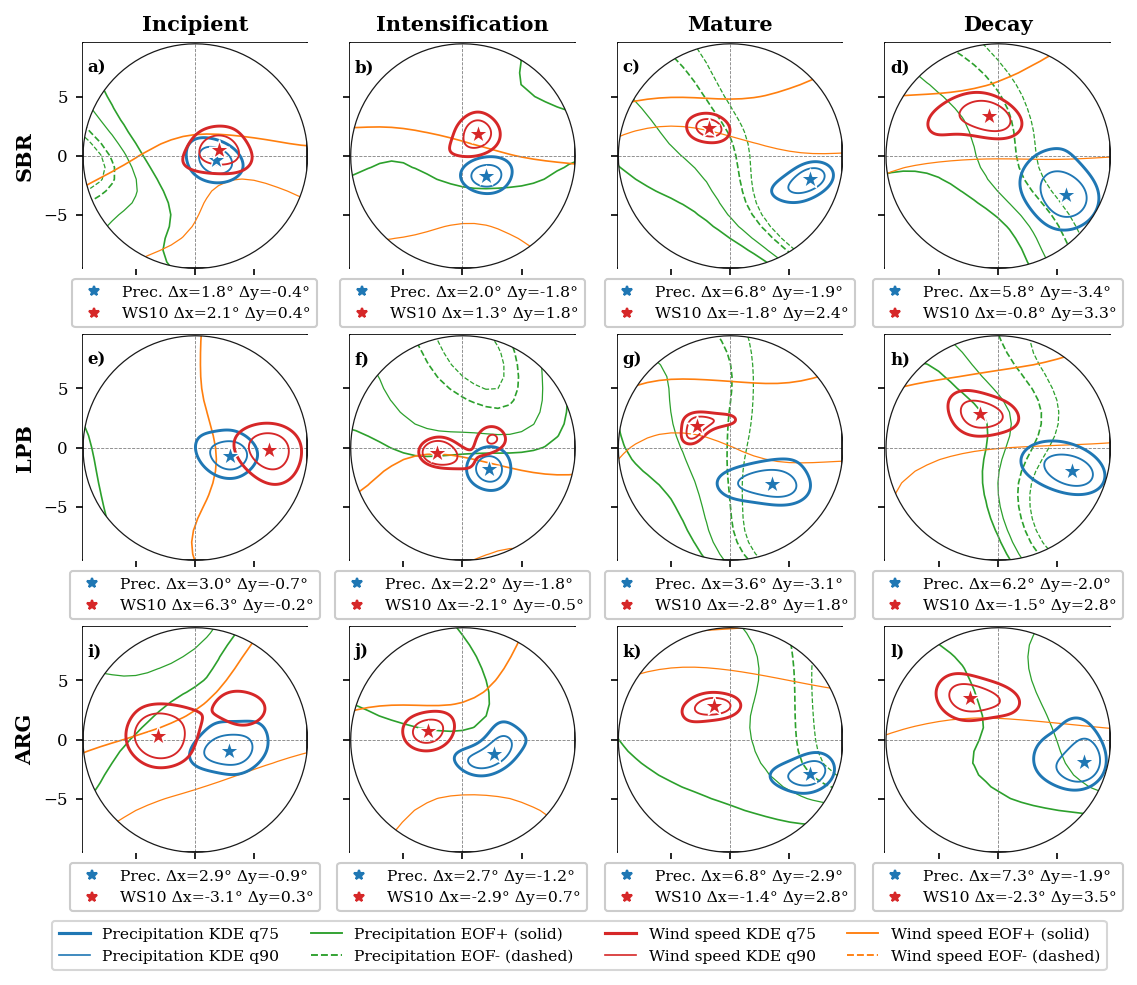
\includegraphics[width=\textwidth]{images/prototipos/prototipo_12panels_p90.png}
\caption[Protótipos estruturais acoplados — Subconjunto p90]{Protótipos estruturais acoplados para o subconjunto de ciclones de alta vorticidade (percentil 90 de vorticidade máxima). O formato dos painéis, a disposição matricial ($3 \times 4$, regiões $\times$ fases), a simbologia de cores e a escala do domínio lagrangiano são idênticos aos da Figura~\ref{fig:prototipo_global}, permitindo quantificar diretamente a transformação estrutural que os sistemas de aprofundamento acelerado experimentam em relação à climatologia geral.}
\label{fig:prototipo_p90}
\end{figure}

A Figura~\ref{fig:prototipo_p90} apresenta os protótipos estruturais acoplados para o subconjunto de ciclones de alta vorticidade (p90). Construída com o mesmo procedimento metodológico da Figura~\ref{fig:prototipo_global} mas restrita ao estrato de sistemas com vorticidade máxima no percentil 90, esta visualização está incluída para quantificar a diferenciação espacial entre os campos de circulação e precipitação nos sistemas de máxima profundificação do Atlântico Sudoeste, fechando o argumento analítico desenvolvido ao longo dos capítulos de precipitação e vento. A comparação direta entre ambas as figuras — possível graças à escala, simbologia e disposição matricial idênticas — permite avaliar se a intensificação dinâmica amplifica ou reorganiza qualitativamente a arquitetura de acoplamento entre variáveis.

O contraste visual com a População Global é imediato e profundo. Na fase de maturidade de SBR (painel c), o PDFe de precipitação (azul) colapsa para uma estrutura compacta e deslocada para leste-sudeste ($\Delta x = 6{,}8^{\circ}$, $\Delta y = -1{,}9^{\circ}$), enquanto o PDFe de vento (vermelho) se concentra no quadrante noroeste ($\Delta x = -1{,}8^{\circ}$, $\Delta y = 2{,}4^{\circ}$). A separação angular entre ambas as modas ultrapassa os $8^{\circ}$ em distância euclidiana, em contraste com os $3^{\circ}$--$4^{\circ}$ observados na População Global. Este padrão de separação cruzada — precipitação a leste-sudeste, vento a noroeste — reproduz-se com notória consistência em LPB (painéis g e h) e, de maneira mais atenuada, em ARG (painéis k e l), onde a precipitação se desloca para leste ($\Delta x = 6{,}8^{\circ}$) e o vento mantém sua posição a noroeste ($\Delta x = -1{,}4^{\circ}$, $\Delta y = 2{,}8^{\circ}$). Esta assinatura geométrica de quadrantes opostos constitui a expressão quantitativa da diferenciação espacial entre campos nos ciclones de máxima profundificação da região.

A gênese dessa diferenciação nos sistemas de alta vorticidade obedece à convergência dos processos de oclusão severa que foram documentados nas análises individuais de cada variável. O padrão de vento a noroeste emerge do ciclo de vida tipo Shapiro-Keyser: a esteira transportadora fria (\textit{cold conveyor belt}, CCB) enrola-se ao redor do núcleo do sistema ocluído, gerando o máximo de circulação de baixo nível no setor posterior esquerdo do vórtice, onde o gradiente de pressão entre o centro de baixa pressão e a crista circundante é mais pronunciado \citep{schultz2021antecedents}. Simultaneamente, a intrusão seca (\textit{dry intrusion}) penetra desde a alta troposfera em direção ao núcleo central do ciclone, erradicando a convecção profunda no domínio central e gerando o característico corredor livre de precipitação (\textit{dry slot}). Como consequência, o remanescente de umidade da WCB é arrastado pela circulação ciclônica em direção à periferia, ficando confinado na frente recuada (\textit{bent-back front}) e formando a banda de precipitação enrolada (\textit{wrap-around precipitation}) no quadrante sudeste e sul \citep{shapiro1990life}. A sobreposição desses dois processos, que operam simultaneamente mas em quadrantes opostos, é precisamente o que gera a configuração de quadrantes diferenciados que o protótipo p90 captura.

A fase de declínio (painéis d, h, l) consolida e exacerba essa separação para os três regimes regionais. Em SBR (painel d), a moda de precipitação se desloca ainda mais para leste ($\Delta x = 5{,}8^{\circ}$, $\Delta y = -3{,}4^{\circ}$) enquanto o vento migra para norte ($\Delta x = -0{,}8^{\circ}$, $\Delta y = 3{,}3^{\circ}$), aumentando a separação euclidiana para mais de $9^{\circ}$. Em LPB (painel h), os contornos PDFe de precipitação se estreitam em uma banda arqueada em direção ao sul-sudeste, enquanto o vento mantém seu núcleo compacto a noroeste, com uma separação modal de $7{,}7^{\circ}$ em latitude. Esse comportamento reflete que, à medida que o ciclone se dissipa, a banda enrolada continua orbitando a margem da intrusão seca mesmo quando o gradiente de pressão geral se enfraquece, enquanto o núcleo de vento se sustenta pela inércia ciclônica e pela advecção de vorticidade remanescente. As cargas do EOF1 de vento (laranja) mantêm sua orientação noroeste-sudoeste em todas as regiões durante o declínio, enquanto as do EOF1 de precipitação (verde) adquirem uma curvatura arqueada em direção ao sul, coerente com a geometria da banda periférica documentada na Seção~\ref{subsubsec:eof1_tp_p90}.

As diferenças regionais no grau de separação refletem a modulação dos forçantes de superfície sobre a dinâmica de oclusão. Em SBR e LPB, o acesso aos fluxos de calor latente oceânico e a forte baroclinicidade favorecem uma oclusão mais rápida, com intrusões secas que penetram profundamente até o núcleo do vórtice e geram a separação mais drástica entre quadrantes \citep{gozzo2013air}. A disponibilidade de umidade tropical canalizada pelo jato de baixos níveis \citep{vera2002cold} sustenta a banda enrolada de precipitação com maior intensidade, aumentando a densidade no quadrante sudeste e alargando a zona de alta probabilidade na maturidade e no declínio. Em ARG (painéis i--l), a oclusão é mais lenta devido à modulação orográfica e à menor disponibilidade de umidade oceânica, gerando uma separação moderada e uma banda de precipitação menos intensa e mais difusa, embora a direção da diferenciação — precipitação a leste-nordeste, vento a noroeste — se mantenha consistente com as outras regiões, revelando que a topologia fundamental da reorganização espacial é universal e que sua intensidade é a variável regionalmente modulada.

A fase incipiente dos ciclones de alta vorticidade (painéis a, e, i) mostra que a diferenciação ainda não está plenamente desenvolvida, mas já exibe uma tendência diferenciada em relação à População Global equivalente. Em SBR (painel a), a moda de vento a noroeste ($\Delta x = 2{,}1^{\circ}$, $\Delta y = 0{,}4^{\circ}$) separa-se da moda de precipitação a leste ($\Delta x = 1{,}8^{\circ}$, $\Delta y = -0{,}4^{\circ}$), com os contornos PDFe ainda parcialmente sobrepostos mas com centros claramente diferenciados. Em LPB (painel e), a separação zonal é mais notável desde o início ($\Delta x_{\text{vento}} = 6{,}3^{\circ}$, $\Delta x_{\text{prec}} = 3{,}0^{\circ}$), refletindo que os sistemas que eventualmente atingirão o percentil 90 de vorticidade já exibem durante sua gênese uma assimetria frontal mais pronunciada do que a média, coerente com o maior gradiente térmico e o maior fluxo de umidade que caracteriza esses ambientes de ciclogênese mais ativos.

% ==============================================================================
% SEÇÃO: DISCUSSÃO
% ==============================================================================
\section{Discussão}\label{sec:discusion_prototipos}

% ------------------------------------------------------------------------------
% PARÁGRAFO 1: Validação da abordagem lagrangiana e comparação com a literatura
% ------------------------------------------------------------------------------

A geometria de co-localização parcial documentada nos protótipos da População Global durante as fases incipiente e de intensificação é coerente com os resultados obtidos por \citet{cardoso2022synoptic} para ciclones subtropicais na região RG1 do Atlântico Sul, que identificaram mediante um quadro lagrangiano similar — com um domínio de $20^{\circ} \times 20^{\circ}$ centrado no vórtice — que as anomalias positivas de vento e precipitação se concentram preferencialmente no setor leste e nordeste do ciclone durante as etapas de desenvolvimento ativo. No entanto, os protótipos do presente trabalho estendem esse resultado de duas maneiras fundamentais: primeiro, ao incorporar explicitamente a fase evolutiva como eixo de estratificação, demonstram que essa co-localização é uma característica das fases iniciais e não uma propriedade estática do ciclone; segundo, ao contrastar a População Global com o subconjunto p90, evidenciam que a co-localização se rompe de maneira sistemática e quantificável precisamente nos sistemas de máxima profundificação dinâmica. Essa distinção não pode ser inferida das análises climatológicas que mediam o ciclo de vida completo \citep{gramcianinov2023impact}, e constitui o valor agregado central da abordagem de protótipos condicionais adotada nesta tese.

% ------------------------------------------------------------------------------
% PARÁGRAFO 2: O desacoplamento espacial em p90 e o modelo Shapiro-Keyser
% ------------------------------------------------------------------------------

A separação de quadrantes nos protótipos p90 — vento a noroeste, precipitação a sudeste e sul — representa a expressão estatística acumulada da transição para o modelo de Shapiro-Keyser documentada para o Atlântico Sul. \citet{gozzo2013air} demonstraram mediante simulações WRF de um ciclone tipo Shapiro-Keyser no Atlântico subtropical que os fluxos de calor latente em superfície são essenciais para sustentar o desenvolvimento da seclusão quente e a intensificação da frente recuada, e que sem esses fluxos a banda de precipitação associada à frente recuada se enfraquece significativamente. Esse resultado tem uma implicação direta para os protótipos p90: a banda de precipitação enrolada que se manifesta no quadrante sudeste é fisicamente insustentável sem o intercâmbio oceânico que caracteriza as regiões SBR e LPB. Isso explica por que em ARG a separação entre quadrantes é quantitativamente menor e a banda de precipitação do protótipo p90 é mais difusa: a menor disponibilidade de calor latente oceânico limita a intensidade da frente recuada e, com isso, a concentração da precipitação enrolada na periferia do vórtice. A convergência entre as conclusões dos experimentos de sensibilidade de \citet{gozzo2013air} e a geometria estatística capturada pelos protótipos valida que a separação de quadrantes observada não é um artefato do processo de média, mas a pegada sistemática de um mecanismo dinâmico bem caracterizado.

% ------------------------------------------------------------------------------
% PARÁGRAFO 3: Comparação com estudos do Hemisfério Norte e transferibilidade 
% do marco conceitual
% ------------------------------------------------------------------------------

A arquitetura de quadrantes documentada nos protótipos p90 do Hemisfério Sul guarda uma correspondência topológica direta, embora especular, com a encontrada em ciclones explosivos do Hemisfério Norte. \citet{priestley2022improved} realizaram composições dos sistemas no topo do 10\% de vorticidade ciclônica no ERA5 aplicando a mesma metodologia de centralização lagrangiana e o mesmo critério de percentil que o presente trabalho, encontrando que os máximos de vento se concentram no quadrante sudoeste do vórtice (equivalente ao noroeste no Hemisfério Sul por inversão da circulação ciclônica), enquanto a precipitação organizada pela WCB se estende para nordeste e sudeste. 

A correspondência geométrica entre o protótipo p90 de SBR e LPB no Atlântico Sul e as composições de \citet{priestley2022improved} no Atlântico Norte é notável em termos da distância euclidiana entre as modas de ambas as variáveis e o grau de contração dos contornos PDFe.

As diferenças observadas — particularmente a maior difusão dos contornos no setor sul e a assimetria meridional mais pronunciada em SBR — são consistentes com a maior disponibilidade de umidade subtropical na região e com a estrutura híbrida que caracteriza muitos dos sistemas p90 do Atlântico Sul, como documentam \citet{evans2012climatology} e \citet{gozzo2014subtropical}. Isso sugere que a diferenciação de quadrantes é um traço universal dos ciclones maduros de alta vorticidade, cuja intensidade regional é modulada pelas condições termodinâmicas do ambiente de gênese.

% ------------------------------------------------------------------------------
% PARÁGRAFO 4: Os protótipos como ferramenta de diagnóstico: vínculo com o marco multivariado
% ------------------------------------------------------------------------------

A abordagem de protótipos estruturais desenvolvida neste capítulo se alinha metodologicamente com propostas recentes que enfatizam a necessidade de vincular explicitamente a evolução dinâmica do sistema com suas manifestações estruturais. \citet{han2025system} propõem um marco de classificação denominado \textit{SyCLoPS} (System Lifecycle of Precipitating Storms) para o Hemisfério Norte, projetado especificamente para estudar a frequência, estrutura e contribuição de precipitação e vento de cada tipo de sistema ao longo de seu ciclo de vida. Assim como o presente trabalho, esse marco reconhece que os ciclones extratropicais não podem ser caracterizados por um único parâmetro de intensidade e que a distribuição espacial de seus campos dinâmicos evolui de maneira não linear durante as diferentes fases. A diferença fundamental reside em que os protótipos aqui apresentados não apenas descrevem a arquitetura do sistema em termos qualitativos, mas a quantificam em um domínio lagrangiano padronizado mediante a sobreposição de densidades de probabilidade espacial e modos dominantes de variabilidade (EOF), gerando representações com um conteúdo probabilístico explícito que permite a comparação direta entre regiões. Essa combinação de geometria modal e densidade probabilística constitui, assim como o marco proposto por \citet{corner2025classification} mediante análise multivariada de parâmetros dinâmicos, um avanço em direção à caracterização objetiva e quantificada dos sistemas de alta vorticidade no Atlântico Sul, uma região onde estudos equivalentes permaneceram até agora muito limitados.

% ------------------------------------------------------------------------------
% PARÁGRAFO 5: Limitações da abordagem e perspectivas futuras
% ------------------------------------------------------------------------------

Duas limitações da abordagem de protótipos merecem discussão explícita. Em primeiro lugar, a padronização do domínio lagrangiano em uma grade fixa de $\pm 9{,}5^{\circ}$ implica que sistemas cuja banda de precipitação enrolada se estende além desse raio — possível nos ciclones de maior escala horizontal — contribuem com densidade PDFe truncada nas bordas do domínio, subestimando a extensão real do campo de precipitação no protótipo. Essa limitação é inerente à abordagem compositiva centrada e foi reconhecida por \citet{cardoso2022synoptic}, que adotaram explicitamente um domínio de $20^{\circ} \times 20^{\circ}$ precisamente para capturar os ventos extremos que podem ocorrer até 500 km do centro do ciclone. Em segundo lugar, a construção dos protótipos sobre o subconjunto estático p90 de vorticidade máxima implica que a amostra inclui sistemas em diferentes fases de seu ciclo de vida no momento de serem catalogados, embora a estratificação por fases mediante o algoritmo \textit{CycloPhaser} \citep{deSouza2025CycloPhaser} mitigue em grande medida esse efeito ao garantir que cada instante analisado pertence à fase correta do ciclone individual. Essas limitações abrem linhas de trabalho futuro: a extensão do domínio para $30^{\circ} \times 30^{\circ}$ para ciclones de grande escala, e a estratificação adicional por velocidade de translado do sistema — um fator que, como apontam \citet{gramcianinov2023impact}, modula diretamente a duração do forçante e a extensão espacial dos campos dinâmicos — permitiriam refinar os protótipos em direção a representações mais completas da diversidade estrutural dos ciclones de alta vorticidade do Atlântico Sul.

% ==============================================================================
\section{Síntese}\label{sec:sintesis_prototipos}
% ==============================================================================

Os protótipos estruturais acoplados sintetizam, em uma representação geométrica única, a evolução diferencial da organização espacial dos campos de precipitação e vento associada aos ciclones extratropicais do Atlântico Sudoeste ao longo de seu ciclo de vida. Na População Global, os campos de precipitação e vento exibem durante as fases incipiente e de intensificação uma co-localização relativa no quadrante oriental, com separações modais moderadas que refletem a organização frontal da WCB como forçante comum. À medida que os sistemas evoluem para a maturidade e o declínio, os campos se separam gradualmente mantendo geometrias difusas que refletem a heterogeneidade estrutural do catálogo geral.

Em contraste, o protótipo p90 revela uma reorganização qualitativa que emerge da oclusão severa. A sobreposição simultânea dos PDFe e EOF1 de ambas as variáveis no mesmo domínio quantifica a diferenciação espacial em sua expressão mais nítida: os sistemas de alta vorticidade maduros e em declínio apresentam os máximos de vento concentrados no quadrante noroeste, dominado pela esteira transportadora fria e pela circulação do vórtice ocluído, enquanto os máximos de precipitação ficam relegados ao quadrante sudeste e sul, confinados na banda enrolada que orbita a margem da intrusão seca. Esta configuração de campos em quadrantes diferenciados, com separações que ultrapassam os $8^{\circ}$--$9^{\circ}$ na maturidade e no declínio de SBR e LPB, constitui a assinatura diagnóstica da estrutura ocluída nesta região e não tem equivalente na População Global.

Do ponto de vista da dinâmica sinótica, este achado implica que os sistemas de alta vorticidade do Atlântico Sul não podem ser caracterizados mediante a co-ocupação simplificada de seus campos de precipitação e circulação.
O centro de máxima variabilidade de precipitação e o centro de máxima variabilidade de vento operam em quadrantes geograficamente opostos em relação ao centro do vórtice, com uma defasagem espacial que se incrementa à medida que o sistema atinge sua máxima profundidade dinâmica.
Em conclusão, os protótipos apresentados neste capítulo constituem a síntese espacial definitiva dos modos de covariância (MEOF) identificados no Capítulo~\ref{chap:meof}. Essa assimetria estrutural reflete a reorganização física do vórtice durante a oclusão, onde a intrusão seca desloca a convecção para a periferia enquanto a esteira transportadora fria consolida a circulação de baixo nível no setor posterior, validando quantitativamente que a separação de quadrantes é a pegada sistemática e previsível da arquitetura dinâmica do ciclone maduro.